\chapter{Polyglot DB Arch}
When designing the data management layer for an application, several of the identified database requirements may be contradictory. Regarding the data model, some data might be of a different structure than other data.

\section{Polyglot Persistence}
Instead of choosing \textit{just one single DBMS} to store the entire data, so-called \textbf{polyglot persistence} could be a viable option to satisfy all requirements towards a modern data management infrastructure.
\begin{itemize}
    \item It denotes that one can choose as many databases as needed so that all requirements are satisfied
    \item Optimal solution when backward-compatibility with a \textbf{legacy application} must be ensured
\end{itemize}
Polyglot persistence however comes with severe \textbf{disadvantages:}
\begin{itemize}
    \item There is no unique query interface or query language, thus there is not a unique database access method
    \item Cross-database consistency is a major challenge, and in case data are duplicated the duplicates have to be updated or deleted in unison
\end{itemize}
It should obviously be avoided to push the burden of all of these query handling and database synchronization task to the application level. Thus the \textit{integration layer} is introduces to take
care of processing queries.
\begin{itemize}
    \item Decomposing queries in to several subqueries
    \item Redirecting queries to the appropriate databases
    \item Recombining the results obtained from the accessed databases
\end{itemize}
Finally the \textit{integration layer} should ensure \textbf{cross-database consistency}: it must synchronize data in the different databases by propagating additions, modifications or deletions among them.
\begin{figure}[!h]
        \centering
        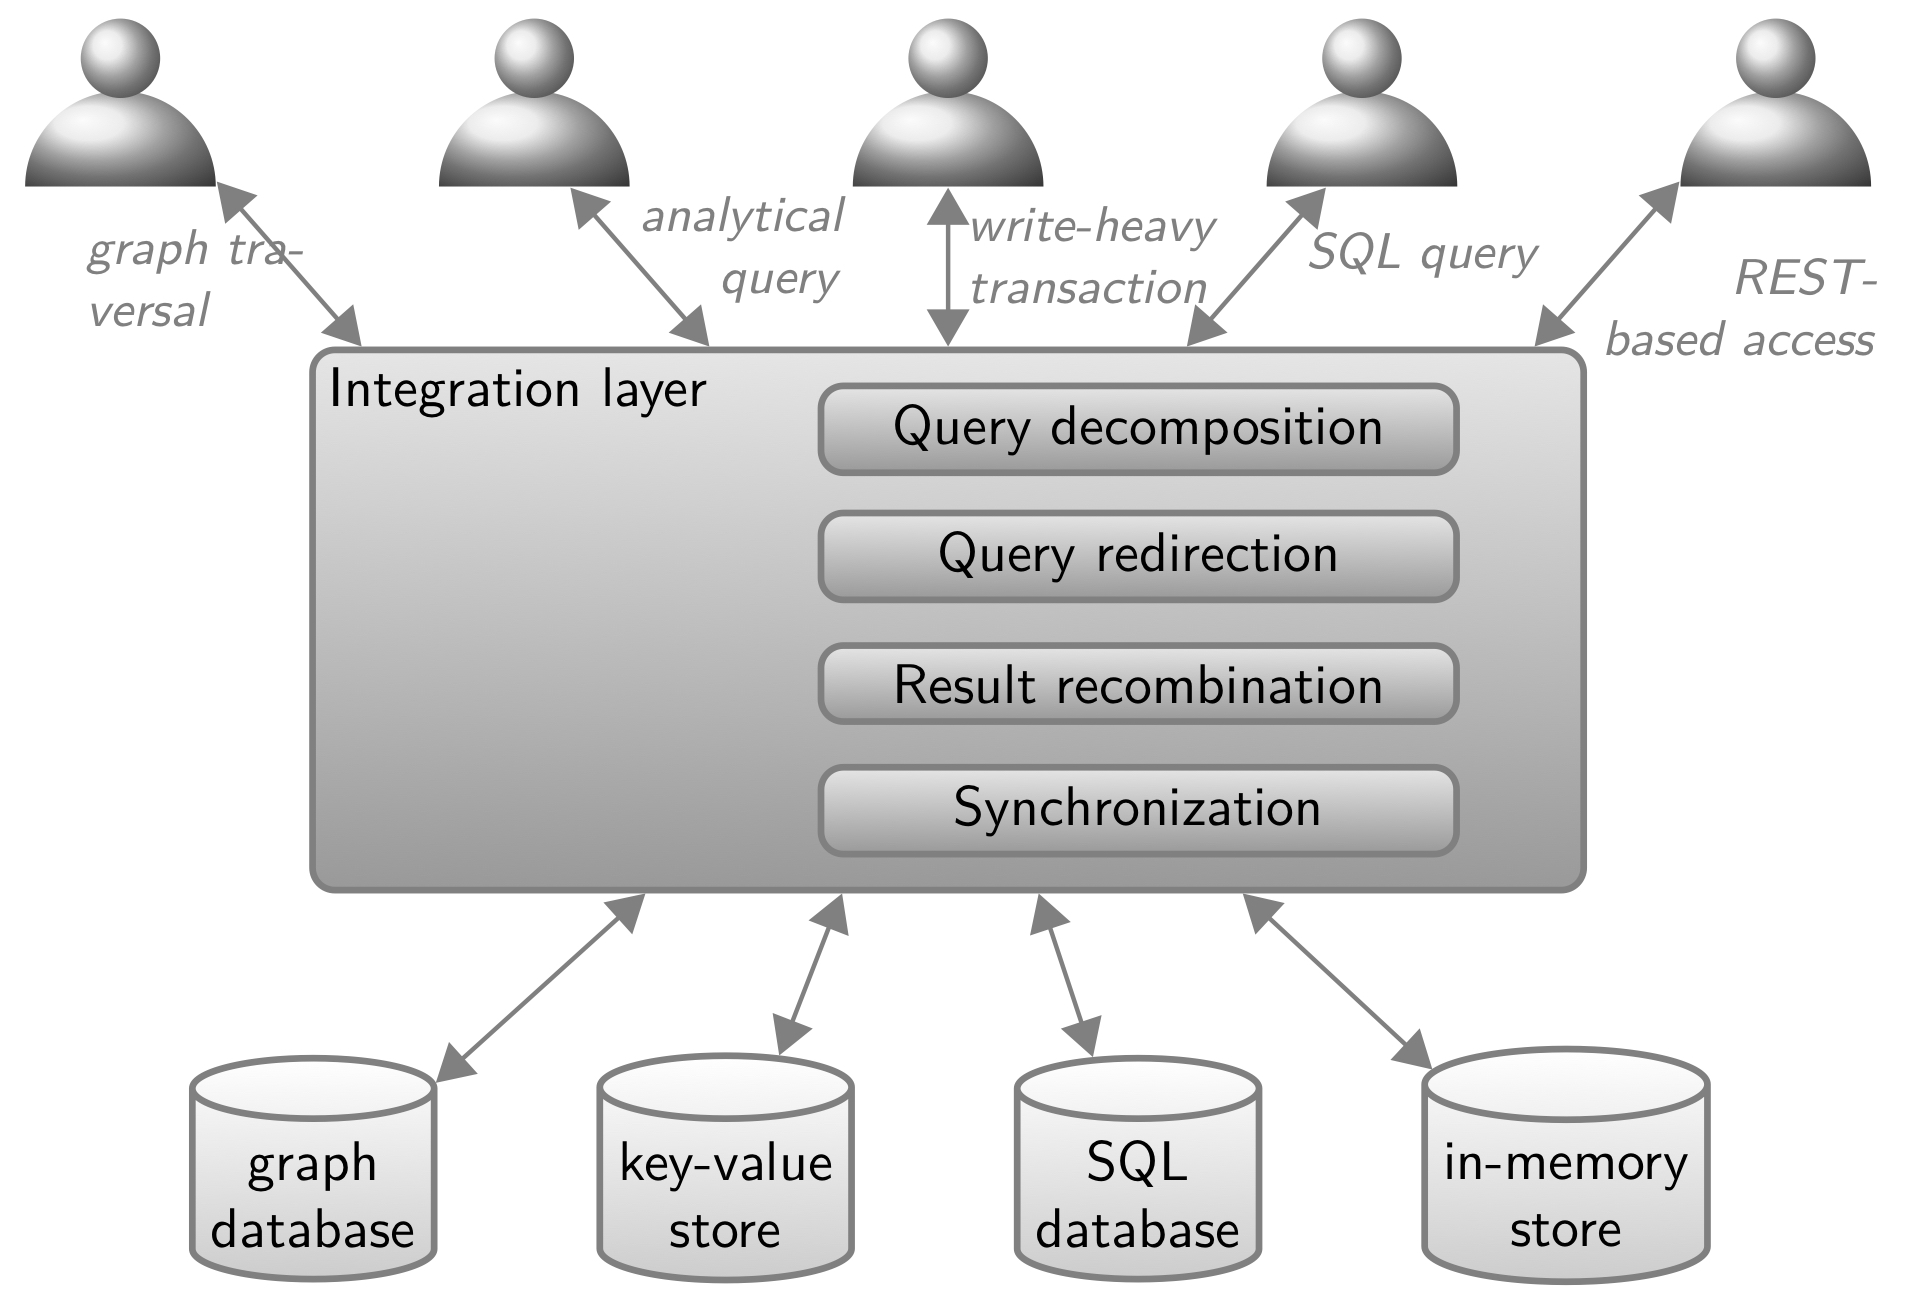
\includegraphics[width=0.7\linewidth]{images/AdvancedDataManagment/polyglot_database_architectures/polygot_pers.jpeg}
        \caption{Polyglot persistence with integration layer}
    \end{figure}


\section{Lambda Architecture}
When real-time (stream) data processing is a requirement, the combination of the following two features might be appropiate:
\begin{itemize}
    \item A slower batch processing layer
    \item A quiker stream processing layer
\end{itemize}
This architecture has been recently termed \textbf{lambda architecture}, it major feature is that it processes a continuous flow of data in the following three layers:
\begin{itemize}
    \item \textbf{Speed Layer} collects only the most recent data and as soon as data ave been included in the other two layers, it can be discarded from the speed layer. Moreover it computes results over its dataset and delivers teh results in several \textbf{real-time views}
    \item \textbf{Batch Layer} stores all data in an append-only and immutable way in a so-called \textit{master dataset}. It evaluates functions over the entire dataset; the results are delivered in so-called \textbf{batch views}
    \item \textbf{Serving Layer} makes batch views accessible to user queries
\end{itemize}
\begin{figure}[!h]
        \centering
        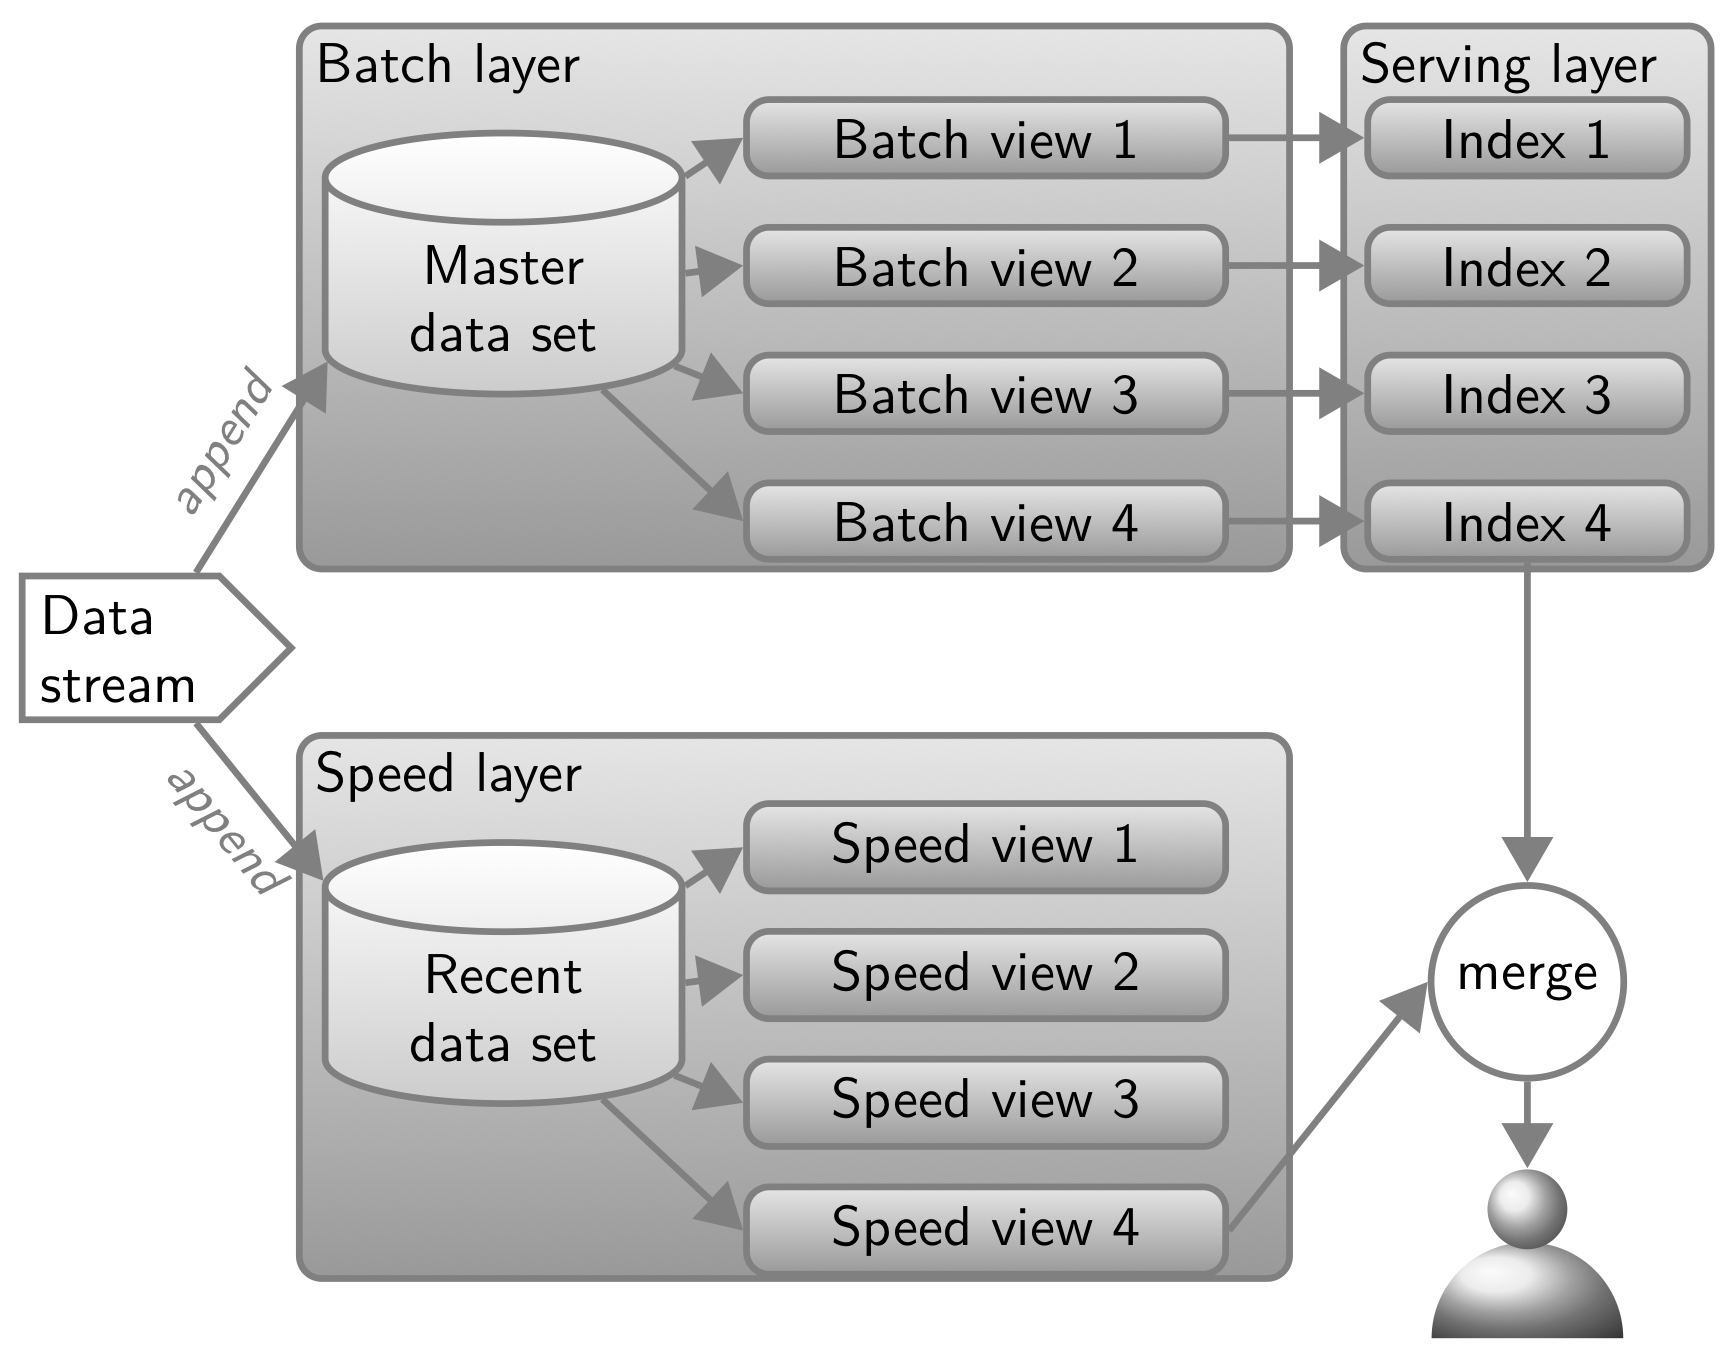
\includegraphics[width=0.7\linewidth]{images/AdvancedDataManagment/polyglot_database_architectures/lambda_arc.jpeg}
        \caption{Lambda architecture}
    \end{figure}


\newpage
\section{Multi-Model Databases}
Relying on different storage backends increases the overall complexity of the system and raises different problems, so it might be advantageous to use a database system that stores data in a single store but provides access to the data with different APIs. 
\begin{tcolorbox}
Databases offering this feature have been termed \textbf{multi-model} databases. They either support different data models directly inside the database engine or they offer layers for additional data models on top of a single-model engine
\end{tcolorbox}
\begin{figure}[!h]
        \centering
        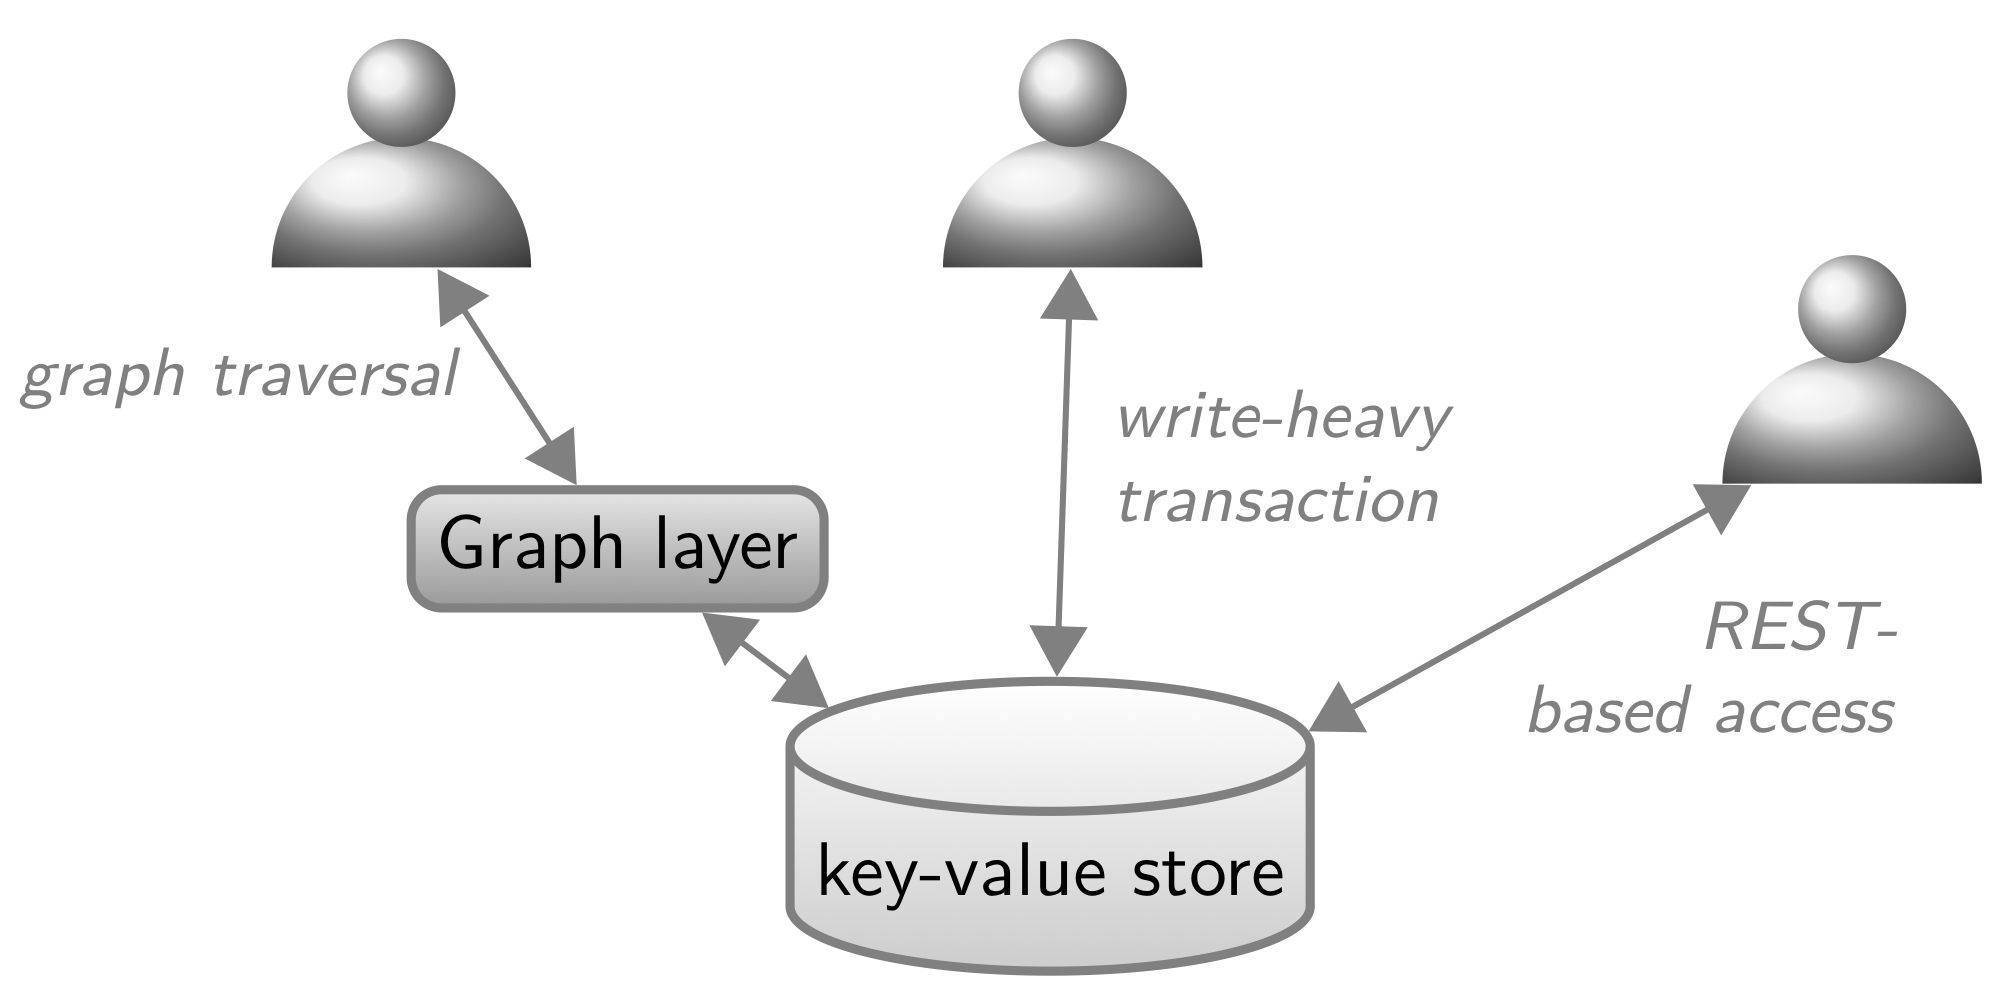
\includegraphics[width=0.7\linewidth]{images/AdvancedDataManagment/polyglot_database_architectures/multimodel_db.jpeg}
        \caption{A multi-model database}
    \end{figure}

Several advantages come along with this single-database multi-model approach:
\begin{itemize}
    \item \textit{Reduced database administration:} maintaining a single database is easier
    \item \textit{Reduced user administration:} only one level of user management is necessary
    \item \textit{Integrated low-level components:} low-level database components can be shared between the different data models in a multi-model database
    \item \textit{Improved consistency:} it is a lot easier to ensure
    \item \textit{Reliability and fault tolerance:} backup just has to be set up for a single database
    \item \textit{Scalability:} data partitioning and data locality can best be configured in a single database system
    \item \textit{Easier application development:} programming efforts regarding database administration  data models and query languages can focus on a single database system
\end{itemize}